\begin{enumerate}
    \item 
    \begin{enumerate}
        \item 
        La longueur des arêtes est de $3$~cm. On sait qu'un pas de lutin mesure $0,05$~cm. 
        
        \medskip
        Donc le lutin devra avancer de : $\dfrac{3}{0,05}=60$ pas.
        
        \begin{scratch}
	
	\initmoreblocks{définir\namemoreblocks{carré}}
	\blockpen{stylo en position d'écriture}
	\blockrepeat{répéter \ovalnum{4} fois}
		{
		\blockmove{avancer de \ovalnum{60}~pas}
		\blockmove{tourner \turnleft~de \ovalnum{90} degrés}
		}
	\blockpen{relever le stylo}	
	\blockmove{avancer de \ovalnum{60}~pas}
	\end{scratch}

        \item $\phantom{X}$\\
        
        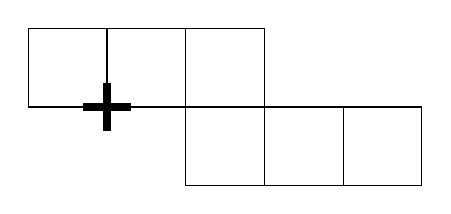
\begin{tikzpicture}
        	\draw (0,0) rectangle (1,1);
        	\draw (1,0) rectangle (2,1);
        	\draw (2,0) rectangle (3,1);
        	\draw (2,0) rectangle (3,-1);
        	\draw (3,0) rectangle (4,-1);
        	\draw (4,0) rectangle (5,-1);
        	\draw[line width=.1cm] (0.7,0) -- (1.3,0) (1,0.3) -- (1,-0.3);
        \end{tikzpicture}
        
	      
	     \item 
        
        \begin{scratch}
            \blockinit{quand\greenflag est cliqué}
            \blockrepeat{répéter \ovalnum{3} fois}
            {
            \blockmoreblocks{carré}
            }
            \blockmove{ajouter \ovalnum{-60} à x}
            \blockmove{ajouter \ovalnum{-60} à y}
            \blockrepeat{répéter \ovalnum{3} fois}
            {
             \blockmoreblocks{carré}
            }
        \end{scratch}
        
    \end{enumerate}
    \item On obtient le patron suivant :\\
    
    \begin{tikzpicture}
    	\draw(0,0) rectangle (1,-1);
    	\draw(1,0) rectangle (2,-1);
    	\begin{scope}[shift={(1,-1)}]
    	  \draw(0,0) rectangle (1,-1);
          \draw(1,0) rectangle (2,-1);
    	\end{scope}
    	\begin{scope}[shift={(2,-2)}]
    	  \draw(0,0) rectangle (1,-1);
          \draw(1,0) rectangle (2,-1);
    	\end{scope}

    \end{tikzpicture}
\end{enumerate}


